\section{Mechanics}
This first part reports on the state of the detectors as we found them
when we removed  them from the field.\\ All of  the antennas had their
metallic   cone  at   least   partly  distorted.    Pictures  in   the
figure~\ref{fig:cone}  show two  extreme cases:  Nono  detector's cone
(shown on  the left) is  distorted, in the  case of Eva (shown  on the
right) the  cone is no longer  attached to the  electronics box.\\ All
the antennas are in a similar state. The mechanics has to be improved.
\begin{figure}[!ht]
  \centering
  \hspace*{-3ex}
  \subfigure{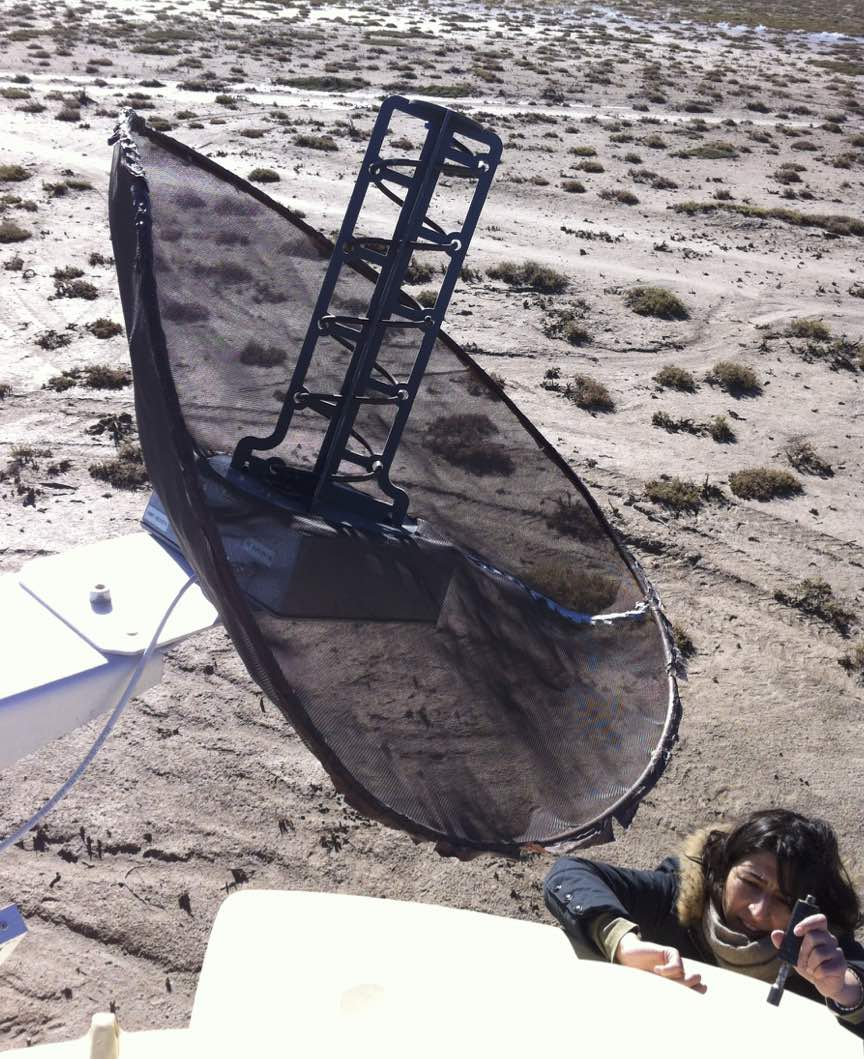
\includegraphics[width=0.49\linewidth]{nono.jpg}}
  \subfigure{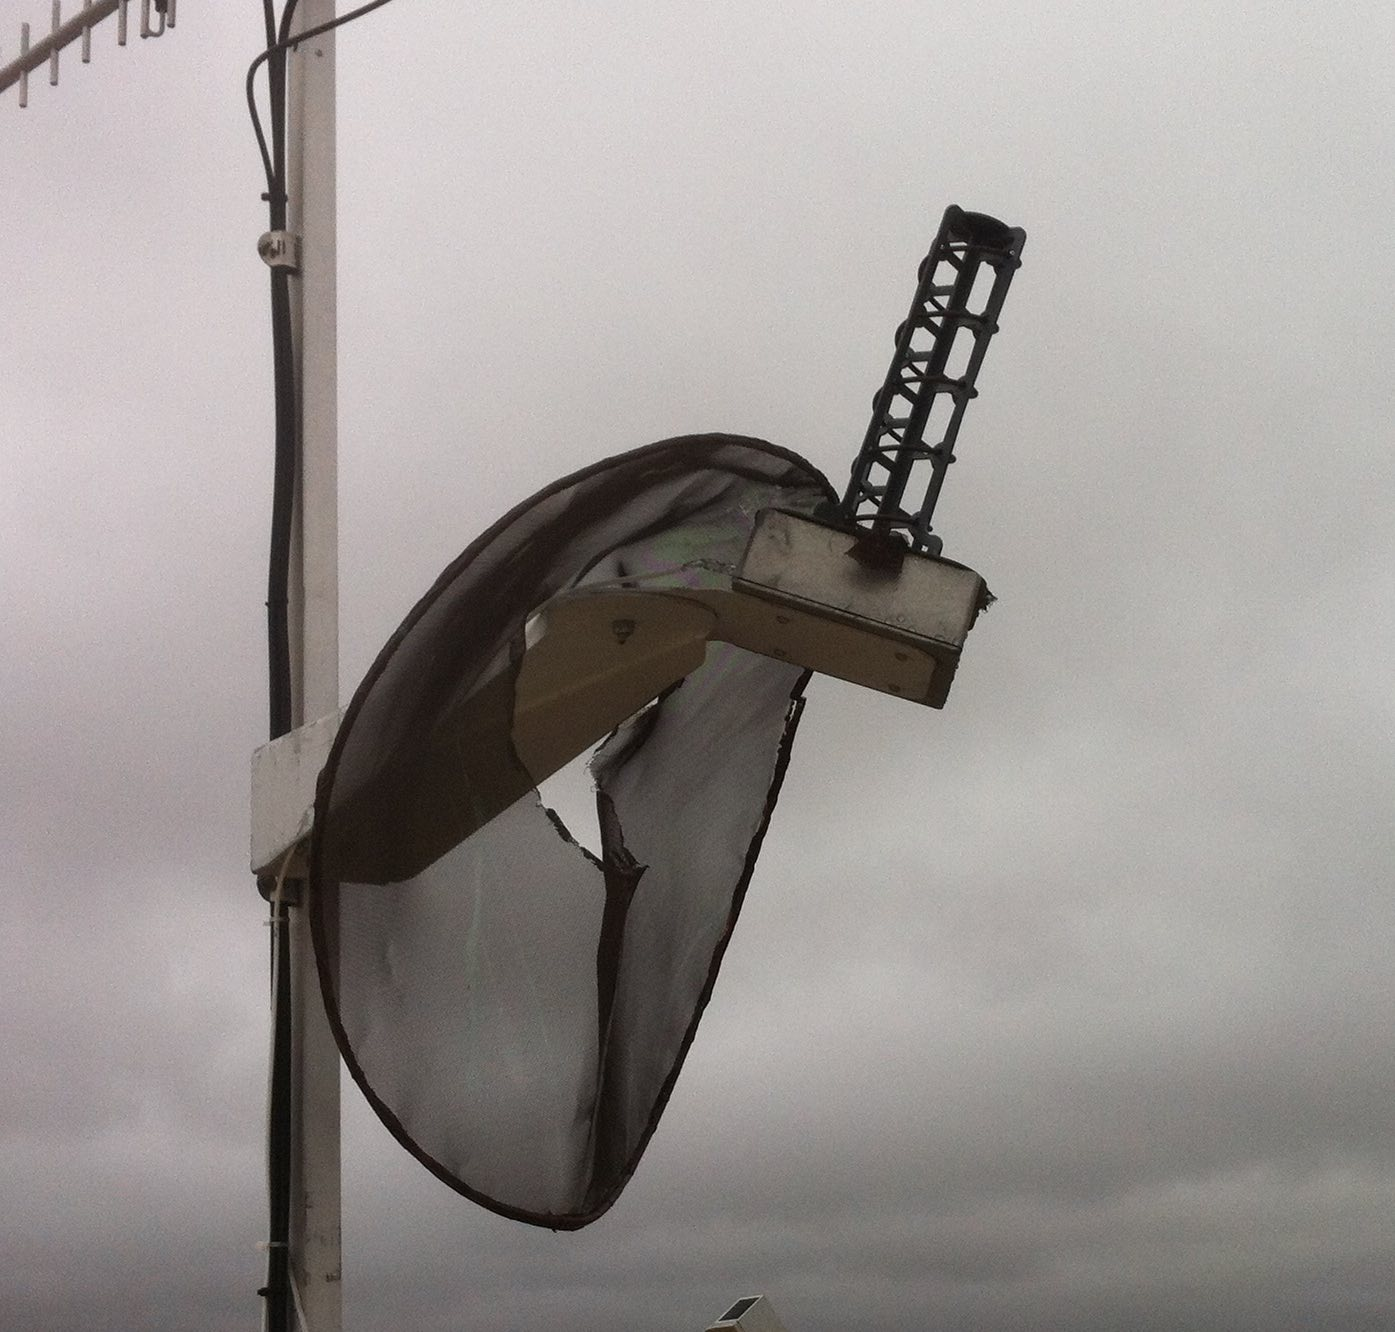
\includegraphics[width=0.49\linewidth]{eva.jpg}}
  \caption{Left:Nono, Right: Eva}
  \label{fig:cone}
\end{figure}

The second  problem encountered was  that water flooded inside  all of
the LNA boxes.   Water went inside the box through the  hole on top of
the box (see figure~\ref{fig:lnabox}  left).  Some boxes had still 1-2
cm  of  water  in  them  and  rust started  to  grow  inside  the  box
(figure~\ref{fig:lnabox} right).

\begin{figure}[!ht]
  \centering
  \hspace*{-3ex}
  \subfigure{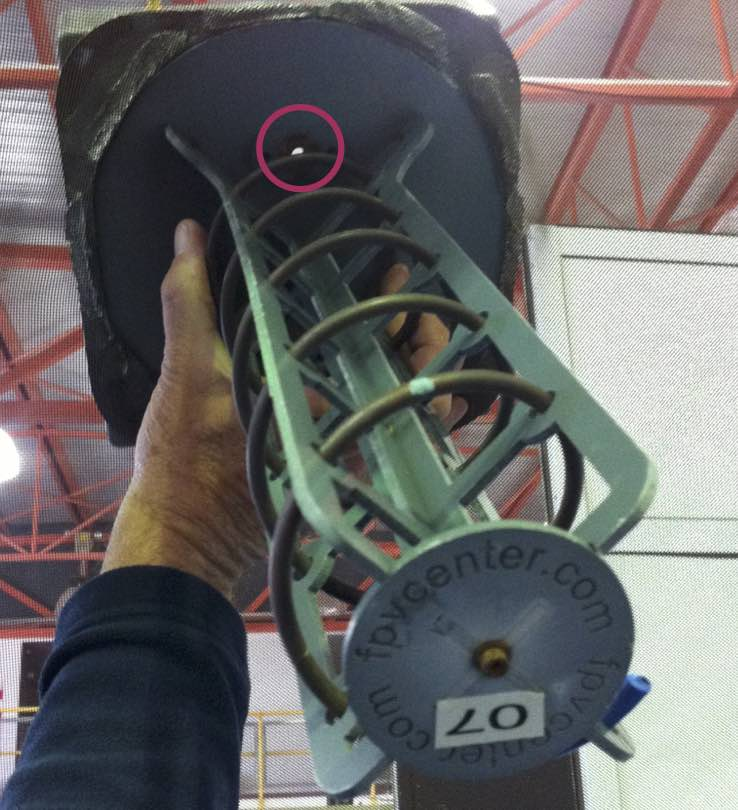
\includegraphics[width=0.49\linewidth]{boitehelix2.jpg}}
  \subfigure{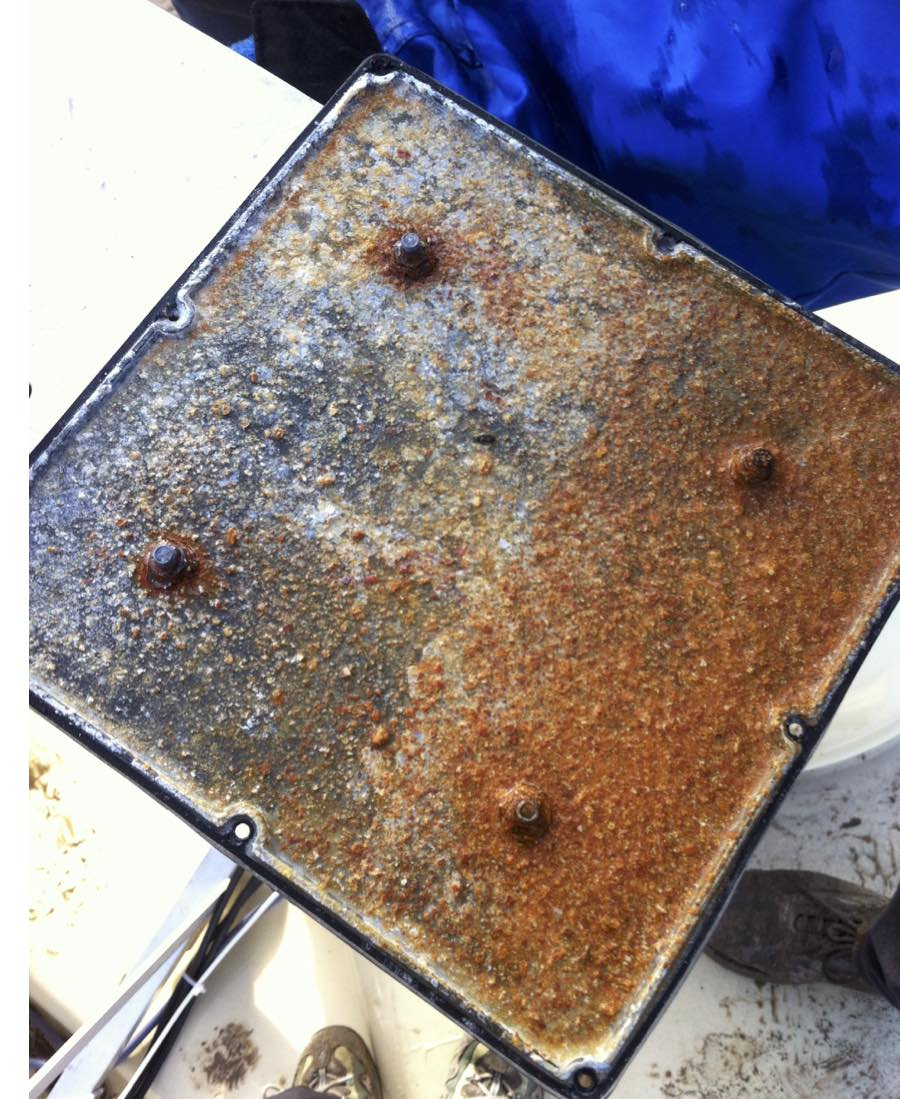
\includegraphics[width=0.49\linewidth]{boxsanty.jpg}}
  \caption{Left: helix antenna, circled the hole where water went into
    the LNA box. Right: rust in Santy's LNA box}
  \label{fig:lnabox}
\end{figure}



